\chapter{Mirrored Arrays}

\section{Overview}

Mirrored arrays use a hybrid approach to replicate data across cluster
nodes and distribute data within each node. It uses shared memory
for caching latency sensitive distributed data structures on Symmetric
Multi-Processor nodes of clusters connected with commodity networks
as illustrated in Figure~\ref{cap:2-D-Array}. The user is responsible
for managing consistency of the data cached within the mirrored arrays.
Instead of applying mirroring to all distributed arrays, the user
can decide, depending on the nature of the algorithm and the communication
requirements (number and size of messages), which arrays can or should
use mirroring and which should be left fully distributed and accessed
without the shared memory cache. 

This hybrid approach is particularly useful for problems where it
is important to solve a moderate sized problem many times, such as
an ab initio molecular dynamics simulation of a moderate size molecule.
A single calculation of the energy and forces that can be run in a
few minutes may be suitable for a geometry optimization, where a few
tens of calculations are required, but is still too long for a molecular
dynamics trajectory, which can require tens of thousands of separate
evaluations. For these problems, it is still important to push scalability
to the point where single energy and force calculations can be performed
on the order of seconds. Similar concerns exist for problems involving
Monte Carlo sampling or sensitivity analysis where it is important
to run calculations quickly so that many samples can be taken.

Mirrored arrays differ from traditional replicated data schemes in
two ways. First, mirrored arrays can be used in conjunction with distributed
data and there are simple operations that support conversion back
and forth from mirrored to distributed arrays. This allows developers
maximum flexibility in incorporating mirrored arrays into their algorithms.
Second, mirrored arrays are distributed within an SMP node (see the
above figure). For systems with a large number of processors per node,
e.g., 32 in the current generation IBM SP, this can result in significant
distribution of the data. Even for systems with only 2 nodes per processor,
this will result in an immediate savings of 50\% over a conventional
replicated data scheme.

%
\begin{figure}
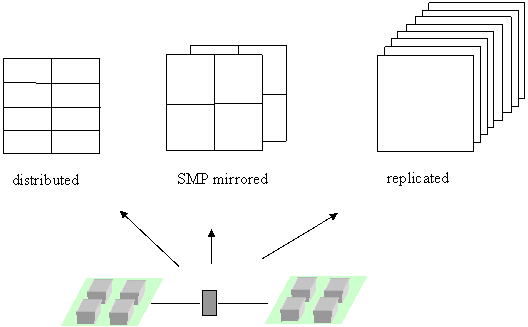
\includegraphics[width=0.9\columnwidth]{mirrored}

\caption{\label{cap:2-D-Array}Example of a two-dimensional array fully distributed,
SMP mirrored, and replicated on two 4-way SMP cluster nodes. }

\end{figure}


The disadvantage of using mirrored arrays is that problems are limited
in size by what can fit onto a single SMP node. This can be partially
offset by the fact that almost all array operations can be supported
on both mirrored and distributed arrays, so that it is easy to develop
code that can switch between using mirrored arrays and conventional
distributed arrays, depending on problem size and the number of available
processors.


\section{Mirrored Array Operations}
\begin{verbatim}
Fortran~integer~\href{http://www.emsl.pnl.gov/docs/global/ga_ops.html\#GA_PGROUP_GET_MIRROR}{ga\_{}pgroup\_{}get\_{}mirror}()~

C~~~~~~~int~\href{http://www.emsl.pnl.gov/docs/global/c_nga_ops.html\#GA_PGROUP_GET_MIRROR}{ga\_{}pgroup\_{}get\_{}mirror}()~

C++~~~~~int~GA::GAServices::pgroupGetMirror()
\end{verbatim}
This function returns a handle to the mirrored processor list, which
can then be used to create a mirrored global array using one of the
NGA\_Create\_{*}\_config calls.
\begin{verbatim}
Fortran~integer~\href{http://www.emsl.pnl.gov/docs/global/ga_ops.html\#GA_MERGE_MIRRORED}{ga\_{}merge\_{}mirrored}(g\_a)~

C~~~~~~~int~\href{http://www.emsl.pnl.gov/docs/global/c_nga_ops.html\#GA_MERGE_MIRRORED}{GA\_{}Merge\_{}mirrored}(int~g\_a)~

C++~~~~~int~GA::GlobalArray::mergeMirrored()
\end{verbatim}
This subroutine merges mirrored arrays by adding the contents of each
array across nodes. The result is that the each mirrored copy of the
array represented by g\_a is the sum of the individual arrays before
the merge operation. After the merge, all mirrored arrays are equal.
This is a collective operation.
\begin{verbatim}
Fortran~integer~\href{http://www.emsl.pnl.gov/docs/global/ga_ops.html\#GA_MERGE_DISTR_PATCH}{nga\_{}merge\_{}distr\_{}patch}(g\_a,~alo,~ahi,~

~~~~~~~~~~~~~~~~g\_b,~blo,~bhi)~

C~~~~~~~int~\href{http://www.emsl.pnl.gov/docs/global/c_nga_ops.html\#GA_MERGE_DISTR_PATCH}{NGA\_{}Merge\_{}distr\_{}patch}(int~g\_a,~int~alo{[}{]},~

~~~~~~~~~~~~~~~~int~ahi{[}{]},~int~g\_b,~int~blo{[}{]},~int~bhi{[}{]})~

C++~~~~~int~GA::GlobalArray::mergeDistrPatch(int~alo{[}{]},~

~~~~~~~~~~~~~~~~int~ahi{[}{]},~int~g\_b,~int~blo{[}{]},~int~bhi{[}{]})
\end{verbatim}
This function merges all copies of a patch of a mirrored array (g\_a)
into a patch in a distributed array (g\_b). This is same as GA\_merge\_mirrored,
except, this function is operated on a patch rather than the whole
array. This is a collective operation.
\begin{verbatim}
Fortran~integer~\href{http://www.emsl.pnl.gov/docs/global/ga_ops.html\#ga_is_mirrored}{ga\_{}is\_{}mirrored}(g\_a)~

C~~~~~~~int~\href{http://www.emsl.pnl.gov/docs/global/c_nga_ops.html\#ga_is_mirrored}{GA\_{}Is\_{}mirrored}(int~g\_a)~

C++~~~~~int~GA::GlobalArray::isMirrored()
\end{verbatim}
This subroutine checks if the array is mirrored array or not. Returns
1 if it is a mirrored array, else it returns 0. This is a local operation. 
